\subsection{Robôs sobre trilhos}
\label{sec::rail}
Na indústria, a automatização de processos de metalização, é
normalmente realizada com a utilização de manipuladores robóticos, pois oferecem
a versatilidade de tarefas e espaço de trabalho possíveis necessários para esse
tipo de aplicação. Entretanto, um sistema composto por um braço robótico capaz
de operar em toda a extensão da superfície de uma pá de uma turbina hidrelétrica
não é compacto, nem móvel o suficiente para ser instalado e desinstalado para a
operação de manuntenção \textit{in-situ}.

A introdução de uma junta prismática acoplada a um trilho é uma estratégia para
reduzir o tamanho e o peso de um manipulador robótico.  Assim, é possível estender o
 espaço de trabalho do robô, sem adicionar peso ao manipulador, uma vez que o
 trilho pode usar as estruturas presentes no ambiente como apoio. 

Na literatura foram encontradas duas soluções para aplicações de manutenção e
inspeção, como solda, específicas para o contexto de turbinas hidráulicas. As
aplicações diferem, principalmente, na estratégia de fixação do sistema
de trilhos.
O Roboturb \cite{roboturb} realiza a fixação
diretamente na pá do rotor, enquanto o robô Scompi \cite{scompi} utiliza um
 trilho fixado em
estruturas adjacentes à pá ou peça a ser reparada.

O Roborturb consiste em um manipulador robótico com seis juntas de revolução e
uma junta primsática acoplada a um trilho flexível, como pode ser observado
na figura \ref{fig::roboturb}, utilizado para o preenchimento de cavidades
geradas por cavitação.
O trilho pode ser conformado e, então, fixado à superfície da pá por meio de um
 sistema passivo de ventosas ou imãs.O robô tem 
a possibilidade de utilizar dois efetuadores distintos, o primeiro consiste em 
um sensor ótico para inspeção do estado de erosão da pá e o segundo consiste em
uma ferramenta de solda do tipo tocha plasma PWH-4A com alimentador automático
de arame, responsável pelo depósito de solda para o preenchimento das cavidades
identificadas pelo sistema.


%TODO Abelha: Posicionar corretamente as figuras
    \begin{figure}[h!]	
		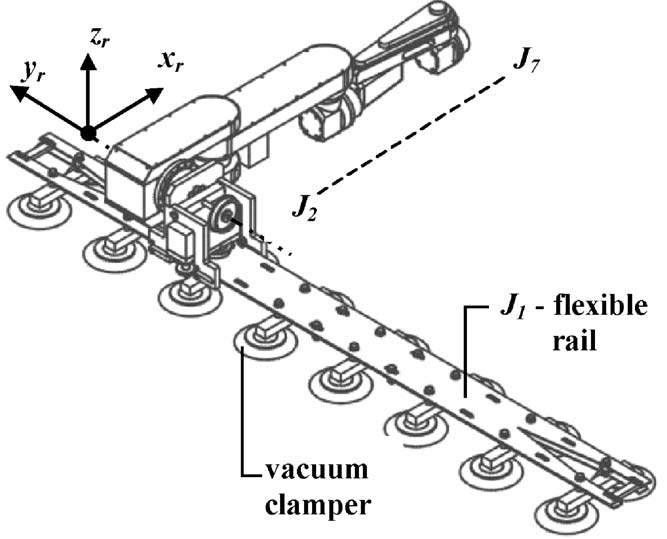
\includegraphics[width=\columnwidth]{figs/trilhos/roboturbpaper}
		\caption{Roboturb - Manipulador robótico sobre trilho flexível}
		\label{fig::roboturb}
	\end{figure}
	\begin{figure}[h!]
		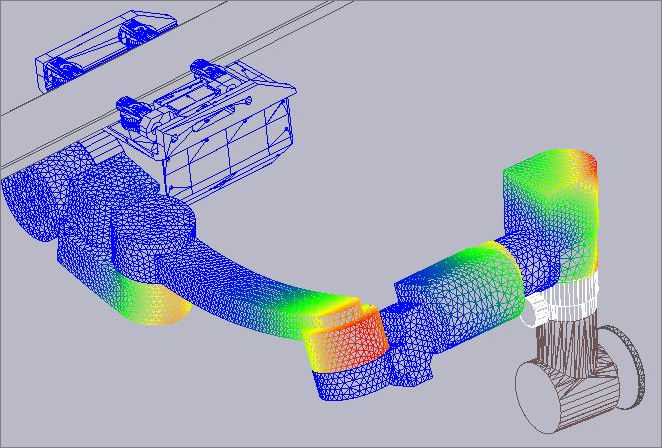
\includegraphics[width=\columnwidth]{figs/trilhos/scompi}
		\caption{SCOMPI - Manipulador robótico sobre trilhos rígidos}
		\label{fig::scompi}
	\end{figure}

Por sua vez, o robô Scompi, fig \ref{fig::scompi}, é um manipulador
multipropósito projetado para realizar reparos em turbinas do tipo \textit{Francis},
 como solda e esmerilhamento das pás. O sistema possuí seis graus de liberdade, sendo 
consitituído por um braço robótico com cinco juntas derevolução e o último grau
 de liberdade proveniente de uma junta prismática que percorre um sistema de 
 trilhos retos ou curvos que são projetados para cada aplicação especificamente. 


Sistemas baseados em trilhos tem como maior benefício a redução do tamanho e,
consequentemente, do peso do manipulador necessário para a execução de tarefas
em um espaço de trabalho que englobe toda a superfície da pá a ser reparada.
Essa redução proporciona facilidade de transporte do robô até o interior da
turbina e também possibilita o projeto de manipuladores que tenham a rigidez
necessária para a realização das tarefas desejadas. Manipuladores
robótico fixos, rígidos o suficiente para aguentar as forças intrínsecas ao
processo de metalização e com espaço de trabalho necessário para trabalhar em
toda a extensão da superfćie da pá seriam muito pesados.
Entretanto, sistemas baseados em trilhos com fixação na própria pá do rotor, necessitam que
o trilho seja movidos caso se deseje que toda a superfície da pá sofra
manuntenção, uma vez que o a área em que o trilho está apoiado não pertence ao espaço de
trabalho do robô. Em adição, sistemas com fixação de trilhos nas estruturas
adjacentes à pá devem atentar as condições para a instalação dispostas pelo
ambiente para equilibrar a relação de custo benefício entre facilidade de
instalação e remoção do trilho e a robustez do mesmo, uma vez que sistemas
permanentes dificilmente são possíveis no contexto das aplicações citadas.

\textbf{Vantagens:}
\begin{itemize}
  \item Redução do tamanho necessário do manipulador;
  \item Redução do peso do manipulador
\end{itemize}

\textbf{Desvantagens:}
\begin{itemize}
  \item Necessidade de instalação e remoção dos trilhos;
  \item Necessidade de movimentação dos trilhos (para trilhos fixados
  diretamente nas pás)
\end{itemize}



